% AI-based Village Pond Planning System - Phase 2 report
\documentclass[11pt,a4paper]{article}

\usepackage[a4paper,margin=19mm,headheight=14pt]{geometry}
\usepackage{graphicx}
\usepackage{xcolor}
\usepackage{amsmath,amssymb}
\usepackage{booktabs,tabularx,array}
\usepackage{enumitem}
\usepackage{fancyhdr}
\usepackage{hyperref}
\usepackage{listings}
\usepackage{caption}
\usepackage{float}
\usepackage{tikz}
\usetikzlibrary{positioning}
\usepackage{parskip}

\definecolor{navy}{HTML}{12304A}
\definecolor{teal}{HTML}{087E8B}
\definecolor{mint}{HTML}{DFF3F2}
\definecolor{pale}{HTML}{F4F8FA}
\definecolor{gold}{HTML}{E5A93D}
\definecolor{ink}{HTML}{1F2933}
\definecolor{muted}{HTML}{52606D}
\definecolor{line}{HTML}{D9E2EC}

\graphicspath{{output/imagegen/}{output/screenshots/}}
\hypersetup{colorlinks=true,linkcolor=teal,urlcolor=teal,citecolor=teal}
\urlstyle{same}
\captionsetup{font=small,labelfont={bf,color=navy},textfont={color=muted}}

\pagestyle{fancy}
\fancyhf{}
\lhead{\textcolor{teal}{AI Village Pond Planning}}
\rhead{\textcolor{muted}{Phase 2 Technical Report}}
\cfoot{\textcolor{muted}{\thepage}}
\renewcommand{\headrulewidth}{0.4pt}
\renewcommand{\headrule}{\hbox to\headwidth{\color{line}\leaders\hrule height \headrulewidth\hfill}}

\setlength{\headheight}{24pt}
\setlist[itemize]{leftmargin=*,itemsep=2pt,topsep=3pt}
\setlist[enumerate]{leftmargin=*,itemsep=3pt,topsep=3pt}
\setlength{\tabcolsep}{5pt}

\lstset{
  basicstyle=\ttfamily\footnotesize,
  backgroundcolor=\color{pale},
  frame=single,
  rulecolor=\color{line},
  framerule=0.5pt,
  columns=fullflexible,
  breaklines=true,
  keepspaces=true,
  showstringspaces=false
}

\newcommand{\sectionrule}{\textcolor{teal}{\rule{\linewidth}{1.2pt}}}
\newcommand{\reportsection}[1]{\section*{\textcolor{navy}{#1}}\sectionrule\vspace{4pt}}
\newcommand{\reportsubsection}[1]{\subsection*{\textcolor{teal}{#1}}}
\newcommand{\code}[1]{\texttt{#1}}
\newcommand{\metric}[1]{\textcolor{teal}{\textbf{#1}}}

\begin{document}

% Cover
\thispagestyle{empty}
\vspace*{-8mm}
\begin{flushright}
\textcolor{teal}{\small\bfseries PHASE 2 \textbar{} TECHNICAL REPORT}
\end{flushright}
\vspace{2mm}

\includegraphics[width=\linewidth,height=77mm,keepaspectratio]{pond-planning-cover.png}
\vspace{5mm}

{\fontsize{28}{32}\selectfont\bfseries\textcolor{navy}{AI-based Village\\Pond Planning System}\par}
\vspace{3mm}
{\large\textcolor{muted}{Contour-map backend API for terrain-derived pond-site and catchment estimation}\par}
\vspace{8mm}

\begin{tabularx}{\linewidth}{@{}X|X@{}}
\textcolor{muted}{\small\bfseries SUBMISSION STATUS} & \textcolor{muted}{\small\bfseries VALIDATION}\\
\textcolor{navy}{\large Backend implementation complete} & \textcolor{navy}{\large 4 automated tests passed}\\
\textcolor{muted}{KML and KMZ upload support} & \textcolor{muted}{Sample contour map analyzed successfully}\\
\end{tabularx}

\vfill
\textcolor{muted}{\small\bfseries REPOSITORY}\par
\url{https://github.com/Galabavamsi/ai-village-pond-planning}\par
\vspace{2mm}
\textcolor{muted}{\small\bfseries VERIFIED API ACCESS}\par
\code{http://127.0.0.1:18000/docs} (SSH-tunnel view from the developer PC)\par
\code{http://10.1.75.53:8000/docs} (private remote host, same network only)\par
\textcolor{muted}{\small Public reverse-proxy URL is not configured in this phase.}\par
\vspace{2mm}
\textcolor{muted}{Prepared for Phase 2 submission \hfill 01 September 2026}
\newpage

\reportsection{1. Executive summary}
This phase delivers a backend API that accepts a contour map in KML or KMZ format and derives terrain-based pond planning information. The service parses contour elevations, builds a local metric elevation grid, routes surface flow using D8 downhill routing, and returns ranked pond candidates with catchment area and GeoJSON geometries.

\noindent\colorbox{mint}{\parbox{\dimexpr\linewidth-2\fboxsep\relax}{\textcolor{navy}{\textbf{Generalization guarantee.} No sample-specific coordinates, locations, or result values are embedded in the implementation. The supplied contour map is used only as a test input.}}}

\reportsubsection{Phase 2 objectives}
\begin{center}
\begin{tikzpicture}[
  node distance=5mm,
  box/.style={draw=teal, rounded corners=2pt, fill=pale, minimum width=31mm, minimum height=17mm, align=center, text=navy, font=\small},
  arrow/.style={->, very thick, teal}
]
\node[box] (upload) {\textbf{1. Upload}\\KML / KMZ};
\node[box,right=of upload] (parse) {\textbf{2. Parse}\\geometry + elevation};
\node[box,right=of parse] (analyse) {\textbf{3. Analyze}\\metric grid + D8};
\node[box,right=of analyse] (return) {\textbf{4. Return}\\JSON + GeoJSON};
\draw[arrow] (upload) -- (parse);
\draw[arrow] (parse) -- (analyse);
\draw[arrow] (analyse) -- (return);
\end{tikzpicture}
\end{center}

The API is structured as an independent analysis service so later phases can add rainfall, government-land availability, soil, satellite imagery, and a frontend map without replacing the core route.

\reportsection{2. Requirements traceability}
\renewcommand{\arraystretch}{1.25}
\begin{tabularx}{\linewidth}{@{}p{30mm}X p{25mm}@{}}
\toprule
\textbf{Requirement} & \textbf{Implementation evidence} & \textbf{Status}\\
\midrule
Backend route & \textbf{POST /analyzeContour}; compatibility alias \textbf{/findCatchment}. & Complete\\
Upload contour map & Multipart upload field \textbf{file}; supports \code{.kml} and \code{.kmz}. & Complete\\
Analyze terrain & Contour parsing, interpolation to an elevation grid, and D8 flow routing. & Complete\\
Identify pond region & Ranks interior cells with high terrain-derived contributing flow and returns a pond footprint. & Complete\\
Estimate catchment & Upstream cells are merged into a GeoJSON Polygon or MultiPolygon with area metrics. & Complete\\
No hard-coding & Coordinates and recommendations are calculated from each uploaded input. & Complete\\
Documentation\\demo & README, this report, OpenAPI docs, automated tests, and sample-map results. & Complete\\
\bottomrule
\end{tabularx}

\reportsection{3. Catchment estimation methodology}
\begin{enumerate}
\item \textbf{Parse KML/KMZ:} extract contour line geometry and elevation from placemark names or supported ExtendedData fields.
\item \textbf{Convert coordinates:} transform WGS84 longitude/latitude into local metre-based coordinates centered on the input extent.
\item \textbf{Interpolate terrain:} use the contour observations to build a regular elevation grid.
\item \textbf{Route flow:} route each cell to its lowest strictly lower neighbour in the eight-cell D8 neighbourhood.
\item \textbf{Accumulate area:} calculate the contributing cell area flowing into every cell.
\item \textbf{Rank candidates:} screen out the boundary, keep cells at or above the 85th percentile of accumulation, and prefer larger contributing area followed by lower elevation.
\item \textbf{Export geometry:} convert the selected point, pond region, and upstream catchment back into WGS84 GeoJSON.
\end{enumerate}

\begin{figure}[H]
\centering

\includegraphics[width=0.92\linewidth]{catchment-terrain-illustration.png}
\caption{Conceptual catchment illustration generated for this report. The actual API derives boundaries from uploaded contours; this image is explanatory, not an analytical output.}
\end{figure}

\reportsubsection{Coordinate handling}
Input coordinates are assumed to be standard WGS84 longitude/latitude as normally stored in KML. The analysis temporarily uses a local equirectangular approximation centered on the input extent so cell areas and flow distances are measured in metres. Returned geometries are converted back to WGS84 GeoJSON for direct map rendering.

\reportsubsection{Design rationale}
A D8 flow model is transparent, reproducible, and extensible for this phase. It gives the frontend a meaningful catchment boundary while keeping later additions independent: rainfall can become a runoff-weighting layer, land ownership can become a constraint mask, and detailed hydrology can replace or refine the routing engine.

\reportsubsection{Core formulas}
Let longitude \(\lambda\), latitude \(\phi\), and the input-centre coordinates \(\lambda_0,\phi_0\) be in radians. Let \(R=6{,}371{,}000\ \mathrm{m}\).

\begin{align}
x &= R\cos(\phi_0)(\lambda-\lambda_0), &
y &= R(\phi-\phi_0). \label{eq:projection}
\end{align}

For grid spacings \(\Delta x\) and \(\Delta y\), the area represented by one cell is
\begin{equation}
A_{\mathrm{cell}} = \left|\Delta x\,\Delta y\right|. \label{eq:cell}
\end{equation}

For cell \(i\), let \(N_8(i)\) be its up-to-eight neighbouring cells and \(z(i)\) its interpolated elevation. D8 routing selects the lowest strictly lower neighbour:
\begin{equation}
f(i) = \underset{n\in N_8(i),\;z(n)<z(i)}{\operatorname{arg\,min}}\;z(n). \label{eq:d8}
\end{equation}
If no such neighbour exists, \(i\) is treated as a local sink.

The contributing area is accumulated from high cells toward lower cells:
\begin{equation}
A(i) = A_{\mathrm{cell}} + \sum_{k:\,f(k)=i} A(k). \label{eq:accumulation}
\end{equation}

For a selected pond cell \(p\), the catchment is the union of all cells that eventually route to \(p\):
\begin{equation}
C(p)=\bigcup_{\text{cells }i\text{ with a flow path to }p} \mathrm{cell}(i). \label{eq:catchment}
\end{equation}
\begin{align}
\mathrm{catchment\_area}_{m^2} &= \operatorname{area}(C(p)),\\
\mathrm{catchment\_area}_{ha} &= \frac{\mathrm{catchment\_area}_{m^2}}{10{,}000}. \label{eq:hectares}
\end{align}

The current phase uses a conservative screening estimate for pond storage:
\begin{align}
d_{\mathrm{pond}} &= \operatorname{clamp}(2.5\,CI,\;1,\;8)\ \mathrm{m},\\
V_{\mathrm{storage}} &= 0.75\,A_{\mathrm{pond}}\,d_{\mathrm{pond}}. \label{eq:storage}
\end{align}
Here \(CI\) is the contour interval in metres and the factor \(0.75\) is a conservative effective-volume factor. In a later rainfall phase:
\begin{equation}
V_{\mathrm{runoff}}=P\,A_{\mathrm{catchment}}\,C_r, \label{eq:runoff}
\end{equation}
where \(P\) is rainfall depth in metres and \(C_r\) is a locally justified runoff coefficient.

\reportsubsection{Algorithm summary}
\begin{lstlisting}
read uploaded KML or KMZ
extract contour geometries and elevation values
project coordinates to local metres around the input centre
interpolate observations onto a regular elevation grid
for every grid cell:
    choose the lowest strictly lower D8 neighbour
    otherwise mark the cell as a sink
sort cells from high elevation to low elevation
accumulate one cell area along each flow target
screen interior cells at or above the 85th accumulation percentile
rank by descending accumulation, then lower elevation
select spatially separated candidates
union all cells flowing to each candidate
return WGS84 GeoJSON and area/storage metrics
\end{lstlisting}

\reportsection{4. API documentation}
\reportsubsection{Endpoint}
\begin{lstlisting}
POST /analyzeContour
Content-Type: multipart/form-data
Field: file=<contour-map.kml|contour-map.kmz>
\end{lstlisting}

\begin{tabularx}{\linewidth}{@{}p{28mm}p{32mm}X@{}}
\toprule
\textbf{Parameter} & \textbf{Type / default} & \textbf{Description}\\
\midrule
\code{grid\_size} & integer / 100 & Cells along the longer map dimension; range 40--220.\\
\code{max\_candidates} & integer / 3 & Number of ranked pond recommendations; range 1--5.\\
\bottomrule
\end{tabularx}

\reportsubsection{Success response}
The JSON response contains analysis status, input contour statistics, terrain-grid metadata, and a list of recommendations. Each recommendation includes a WGS84 point, pond region, elevation, depth/storage estimate, and a catchment object with area in square metres/hectares and GeoJSON geometry.

\begin{lstlisting}
{
  "analysis": {"status": "completed", "algorithm_version": "terrain-d8-v1"},
  "input": {"contour_features": 2710, "contour_interval_m": 1.0},
  "recommendations": [{
    "site_id": "pond-1",
    "location": {"type": "Point",
                 "coordinates": [81.2899372847, 21.2499875606]},
    "catchment": {"area_hectares": 16.0327,
                  "geometry": {"type": "MultiPolygon"}}
  }]
}
\end{lstlisting}

\reportsubsection{Additional routes and errors}
\textbf{GET /health} returns service status. \textbf{GET /docs} opens interactive Swagger UI. \textbf{POST /findCatchment} is a compatibility alias. The API returns 415 for unsupported extensions, 413 for files over 75 MB, 400 for empty uploads, and 422 for invalid or unusable contour maps.

\reportsection{5. Demonstration using the supplied contour map}
Test input: \code{contour-maps/contours\_1m.kml} (approximately 6.7 MB). The endpoint was exercised through HTTP and returned status 200.

\begin{tabularx}{\linewidth}{@{}X r@{}}
\toprule
\textbf{Observed metric} & \textbf{Result}\\
\midrule
Contour features & 2,710\\
Elevation range & 267--298 m\\
Contour interval & 1 m\\
First recommended point & \code{81.2899372847, 21.2499875606}\\
First estimated catchment & 16.0327 hectares\\
First storage estimate & 4,233.98 \(\mathrm{m^3}\)\\
\bottomrule
\end{tabularx}

\reportsubsection{Reproduce locally}
\begin{lstlisting}[language=bash]
python run.py
curl -X POST "http://127.0.0.1:8000/analyzeContour?grid_size=100&max_candidates=3" \
  -F "file=@contour-maps/contours_1m.kml"
\end{lstlisting}
The interactive alternative is \code{http://127.0.0.1:8000/docs}: expand \textbf{POST /analyzeContour}, select \textbf{Try it out}, upload the KML, and execute the request.

\begin{figure}[H]
\centering

\includegraphics[width=0.9\linewidth]{rural-pond-conservation.png}
\caption{Conceptual rural rainwater-harvesting visual generated for this report. It provides context for the planning problem; the API evidence is shown in the following screenshots.}
\end{figure}

\reportsection{6. Interactive Swagger UI evidence}
The screenshots document the complete demonstration flow: available routes, selected sample file, and successful HTTP 200 response.

\begin{figure}[H]
\centering

\includegraphics[width=0.94\linewidth]{01_swagger_api_overview.png}
\caption{Swagger UI overview showing the health check and contour-analysis routes.}
\end{figure}

\begin{figure}[H]
\centering

\includegraphics[width=0.94\linewidth]{02_swagger_upload_form.png}
\caption{Expanded POST /analyzeContour form with the sample KML selected and Execute button ready.}
\end{figure}

\begin{figure}[H]
\centering

\includegraphics[width=0.94\linewidth]{03_swagger_success_response.png}
\caption{Successful HTTP 200 response showing completed analysis, contour statistics, terrain grid, and recommendation JSON.}
\end{figure}

The response can be consumed directly by a frontend map because pond and catchment geometries are returned as WGS84 GeoJSON.

\reportsection{7. Validation and deployment}
\begin{tabularx}{\linewidth}{@{}p{35mm}X p{22mm}@{}}
\toprule
\textbf{Test} & \textbf{Purpose} & \textbf{Result}\\
\midrule
Health route & Confirms service responds. & Passed\\
Sample KML analysis & Confirms the full terrain pipeline. & Passed\\
Unsupported extension & Confirms upload validation. & Passed\\
Sample KMZ analysis & Confirms archive extraction. & Passed\\
\bottomrule
\end{tabularx}

\reportsubsection{Remote deployment}
\begin{lstlisting}[language=bash]
git clone https://github.com/Galabavamsi/ai-village-pond-planning.git
cd ai-village-pond-planning
python3 -m venv .venv
source .venv/bin/activate
pip install -r requirements.txt
tmux new -s pond-api
uvicorn app.main:app --host 0.0.0.0 --port 8000
\end{lstlisting}
The remote process is running in tmux session \code{pond-api}. The verified health response reports service status \code{ok} for \code{pond-planning-api}. The developer-PC tunnel exposes the same remote service at \code{http://127.0.0.1:18000}. A reverse proxy or secure tunnel is still required for a public evaluator URL. SSH credentials and tokens must remain outside the repository.

\newpage
\reportsection{8. Limitations and future phases}
The current result is a terrain-only planning estimate, not a final civil-engineering design. The reported storage estimate uses a conservative compact footprint and depth approximation derived from contour interval. It does not yet model rainfall intensity, runoff coefficient, infiltration, evaporation, land ownership, soil, structures, or field constraints.

\begin{tabularx}{\linewidth}{@{}p{35mm}X@{}}
\toprule
\textbf{Future layer} & \textbf{Planned extension}\\
\midrule
Rainfall & Apply rainfall and runoff coefficients to convert catchment area into seasonal volume scenarios.\\
Government land & Intersect candidate pond/catchment geometries with land-ownership boundaries.\\
Satellite data & Add land cover, drainage, vegetation, and water-body constraints.\\
Hydraulic design & Replace approximate footprint/depth with a stage-area-volume model.\\
Frontend map & Render returned GeoJSON on an interactive map and expose analysis parameters.\\
\bottomrule
\end{tabularx}

\vfill
\begin{center}
\textcolor{muted}{\small Conceptual AI-generated images are clearly identified; analytical claims are based on the implementation, tests, and captured API response.}
\end{center}

\end{document}
